\documentclass[conference]{IEEEtran}
\usepackage[T1]{fontenc}
\usepackage{graphicx}
\usepackage{booktabs}
\usepackage{amsmath}
\usepackage{multirow}
\usepackage{xcolor}
\usepackage{url}
\usepackage[hidelinks]{hyperref}
\hypersetup{pdftitle={Museum Scans Are Close to WikiArt},pdfauthor={Abdullahi Jimale}}
\usepackage{cite}

% ---------------------------------------------------------------------------
% Results that come from notebooks/final_extras.ipynb (CORAL, grayscale-augmentation training).
% Replace "--" with the numbers in wikiart_runs/final_extras/{coral_report,grayaug_report}.txt.
\newcommand{\pend}{--}
% ---------------------------------------------------------------------------

\newcommand{\pp}{\,pts}
\begin{document}

\title{Museum Scans Are Close to WikiArt: Style Transfer from WikiArt to the Met and the Rijksmuseum, and Why Knowing the Artist Matters More}

\author{\IEEEauthorblockN{Abdullahi Jimale}
\IEEEauthorblockA{CIS 631, Department of Computer Information Science\\
Minnesota State University, Mankato\\
Instructor: Dr.~Suboh Alkhushayni\\
Code and data: \url{https://github.com/abdull254/wikiart-to-museum}}}

\maketitle

\begin{abstract}
Art-style classifiers are trained and tested on WikiArt, but museums would use them on their own collection images. We ask two separate questions. \textbf{RQ1:} how much does a classifier trained only on WikiArt lose on professional museum digitizations from the Metropolitan Museum of Art (937 paintings) and the Rijksmuseum (3,092)? \textbf{RQ2:} does fine-tuning on 5--50 paintings per style from one museum help on the other? We use six historical styles, an artist-disjoint WikiArt split, and museum test sets with every WikiArt overlap removed. The loss is small. For an ImageNet-initialized ResNet-50 (3 seeds), top-1 balanced accuracy on painters never seen in training is 61.1\% on WikiArt test, 57.5\% at the Met and 58.2\% at the Rijksmuseum; for a CLIP linear probe it is 70.9\%, 68.2\% and 66.4\%. With a painter-level bootstrap every museum gap has a 95\% interval that includes zero, and the upper 90\% bound is below 10 points for every model, although the test sets are too small to show equivalence within $\pm$5 points. Knowing the artist matters more than the image source: paintings by artists seen in training score about 12 points higher at the Met for all three models. A few museum paintings do not transfer: none of 24 few-shot gains is significant. Errors concentrate at style boundaries and in label definitions (for example, Dutch Mannerism is not the Italian Mannerism WikiArt teaches), not in digitization artifacts. Merging styles into three eras raises balanced accuracy to 87--91\%, which we report next to, not instead of, the six-style results.
\end{abstract}

\begin{IEEEkeywords}
art style classification, domain shift, WikiArt, museum collections, transfer learning, CLIP, few-shot learning
\end{IEEEkeywords}

% ===========================================================================
\section{Introduction}

Automatic style recognition could help museums tag collections and help visitors search them. Nearly all style classifiers are trained and tested on WikiArt~\cite{karayev2014,saleh2016,tan2016,cetinic2018,zhao2021,zhao2022}, a web collection of reproductions with community style tags. A WikiArt test score says how well a model works on WikiArt; it does not say how well it works on a museum's own images. Deep models are known to be brittle when the visual domain changes~\cite{castellano2021,gulrajani2021}, so a drop on museum images is a reasonable expectation.

This project tests that expectation. The idea and its two-question framing come from classmates Mashfika Jahan and Yisihaq Yemiu, who proposed it in their own course proposal and shared it with their agreement~\cite{jahan2026}. Following their framing, we keep two claims apart:
\begin{itemize}
\item \textbf{RQ1 (transfer).} How much does performance change when a model trained only on WikiArt is tested on the Met and the Rijksmuseum?
\item \textbf{RQ2 (few-shot recovery).} Does fine-tuning on $k = 5, 10, 25, 50$ paintings per style from one museum improve results at the other museum, in both directions?
\end{itemize}

We expected a large gap and found a small one. That is the main finding. The museum images we test are \emph{professional collection digitizations}: evenly lit, straight-on, color-calibrated scans cropped to the painting. They are not photographs taken in the gallery, and we make no claim about visitor photos. Within that domain, our results say:
\begin{enumerate}
\item The WikiArt-to-museum gap is small for every model: 2--5 points of balanced accuracy, with 95\% intervals that include zero (Section~\ref{sec:rq1}).
\item Artist familiarity matters more than image source. At the Met, paintings by artists seen in WikiArt training score about 12 points higher than paintings by unseen artists, for a fine-tuned CNN and for two frozen foundation models.
\item A few labeled museum paintings do not transfer to the other museum (RQ2).
\item Most confident errors come from style boundaries and from how the two label sources define style, not from digitization artifacts. The weakest class, Rijksmuseum Mannerism, is mostly Dutch Mannerism, while WikiArt's Mannerism is mostly Italian.
\end{enumerate}

\textbf{Contribution.} To our knowledge this is the first test of style transfer from WikiArt to museum digitizations from two separate collections with artist-disjoint training data, overlap-removed museum test sets, painter-level statistics and a few-shot test in both directions. We release code, splits, object IDs, label maps and every result file.

% ===========================================================================
\section{Related Work}

\textbf{Style classification on WikiArt.} Karayev et al.~\cite{karayev2014} introduced WikiArt style recognition; Saleh and Elgammal~\cite{saleh2016} and Tan et al.~\cite{tan2016} set early baselines, the latter defining the widely used 27-style release. Cetini\'c et al.~\cite{cetinic2018} showed that fine-tuning ImageNet CNNs works well for style, genre and artist, and Zhao et al.\ compared architectures~\cite{zhao2021} and large-scale transfer (BiT)~\cite{zhao2022}. Recent ensembles reach 68.6\% on 21 classes~\cite{menis2024}, but with random splits that share artists between train and test. Ashton~\cite{ashton2026} showed on the same WikiArt release we use that accuracy falls from 86.9\% to 76.6\% when artists are held out, so random-split numbers partly measure artist recognition. \emph{We use an artist-disjoint split throughout and test outside WikiArt.}

\textbf{Transfer across art collections.} Sabatelli et al.~\cite{sabatelli2018} already asked whether models fine-tuned on one art collection transfer to heritage objects from a different dataset, and found that fine-tuning, not off-the-shelf features, is needed. The Rijksmuseum Challenge~\cite{mensink2014} and the Met dataset~\cite{ypsilantis2021} benchmark recognition inside one collection, and Koniusz et al.~\cite{koniusz2018} studied studio-to-gallery photo shift for exhibit identification. Kipke et al.~\cite{kipke2026} compared WikiArt with Wikidata images of the same artists and found small differences. \emph{We study style, not instance recognition, and test transfer from WikiArt to two museums with overlapping works removed.}

\textbf{Domain generalization and adaptation.} Domain shift is usually handled by aligning feature distributions, adversarially (DANN~\cite{ganin2016}) or by matching second-order statistics (CORAL~\cite{sun2016coral,sun2016deepcoral}); careful benchmarks show that plain empirical risk minimization is hard to beat~\cite{gulrajani2021}. Shifts in class frequency (label shift) need different corrections~\cite{lipton2018}. Castellano and Vessio's survey~\cite{castellano2021} notes that art models are brittle across visual domains. \emph{Our museum problem is one instance of this pattern; we separate label shift from image shift and use CORAL as the adaptation baseline.}

\textbf{Foundation and vision-language models for art.} Strafforello et al.~\cite{strafforello2024} evaluated CLIP and large vision-language models zero-shot on WikiArt and JenAesthetics; CLIP zero-shot style accuracy was low and famous works may be in pretraining data. Asperti et al.~\cite{asperti2025} found CLIP's style recognition on National Gallery of Art images moderate, with Romanticism among the most confused styles, and Kipke et al.~\cite{kipke2026} benchmarked CLIP, SigLIP and DINOv2 on WikiArt. \emph{We compare a fine-tuned CNN with frozen CLIP, DINOv2 and SigLIP features on the same artist-disjoint, museum-shifted test, and treat pretraining contamination as a threat to validity.}

\textbf{Gap.} We searched arXiv and the web (2024--2026) for art style classification combined with WikiArt, museum, domain shift, CLIP, DINOv2 and artist-disjoint. We found no study that trains on WikiArt and tests \emph{style} on museum digitizations from two separate collections with artist-disjoint, overlap-removed test sets.

% ===========================================================================
\section{Data}

\begin{figure*}[t]
\centering
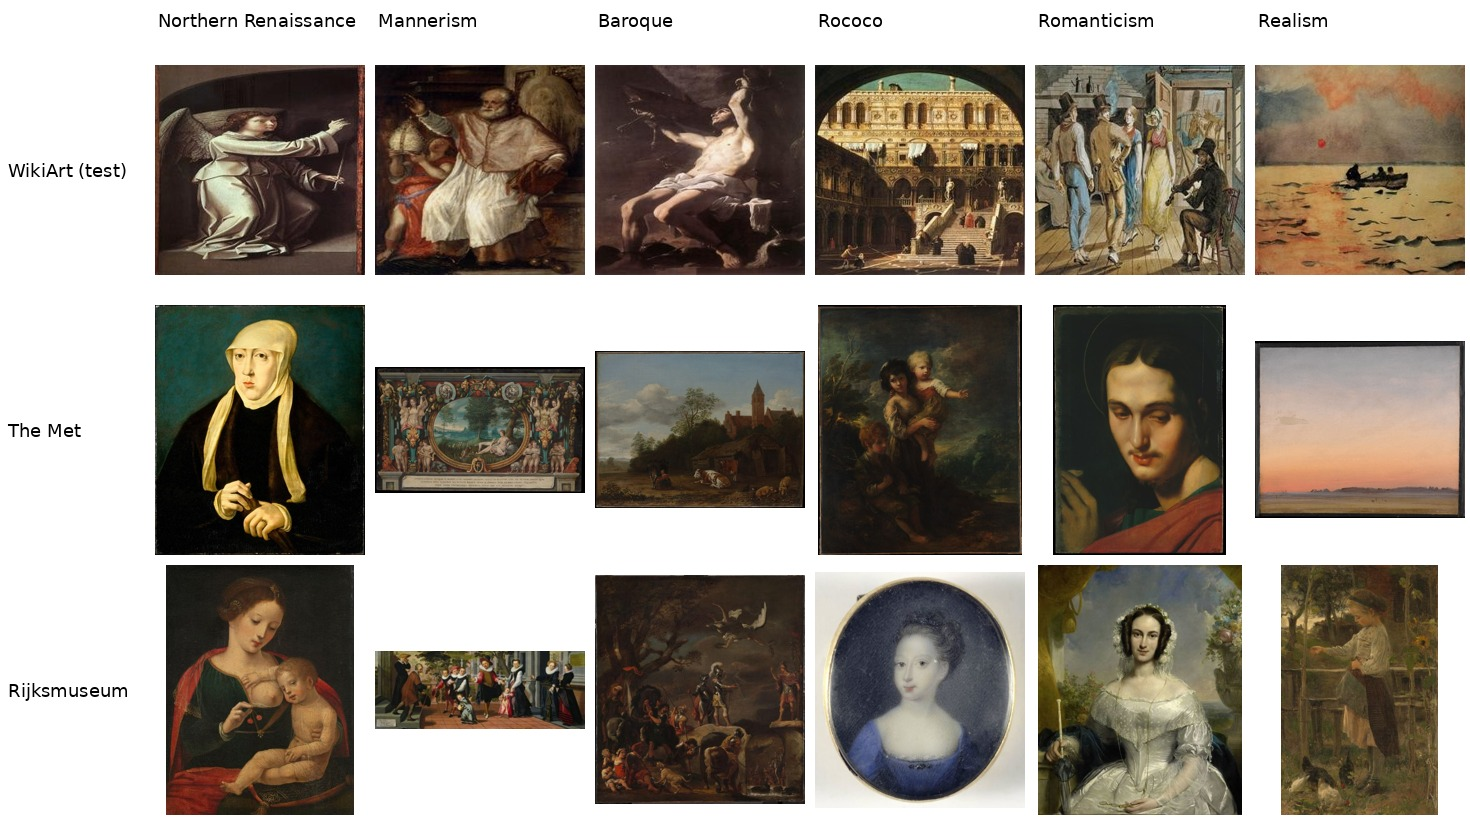
\includegraphics[width=0.92\textwidth]{figures/examples.jpg}
\caption{One random painting per style from WikiArt test and from each museum's unseen-artist test set. Museum images are professional digitizations; some keep a thin border, an oval or arched format, or a visible frame, which WikiArt's square crops hide.}
\label{fig:examples}
\end{figure*}

\textbf{Sources.} WikiArt comes from the Hugging Face release \texttt{Artificio/WikiArt\_Full}~\cite{wikiartfull} (103,250 images), chosen because every image has an artist; the common 27-style release does not, which rules out an artist-disjoint split. The Met set comes from the Met Collection API~\cite{metapi} (European Paintings and the Robert Lehman Collection, public-domain only, 2,214 paintings). The Rijksmuseum set comes from the Rijksmuseum Search API with IIIF images~\cite{rijksapi} (paintings collection, \texttt{SK-} numbers, 4,695 paintings). Both museums were harvested on 2026-10-20; object IDs are released.

\textbf{Styles and labels.} Neither museum records a style. We derive one with numbered rules (Table~\ref{tab:rules}): the artwork's Wikidata movement (R1), the painter's Wikidata movement (R2a--c), and a date rule (R7) only for periods with one dominant style (1400--1599 Renaissance split by region, 1600--1719 Baroque, 1720--1779 Rococo). Paintings from 1780 on with no movement are left unlabeled, and since Oct.~26 a movement that does not fit the painting's date is dropped. Styles needed at least 200 WikiArt images and 30 per museum, leaving six: Northern Renaissance, Mannerism (Late Renaissance), Baroque, Rococo, Romanticism and Realism.

\textbf{Label check.} One hundred labels (50 per museum) were reviewed in two steps. First, an AI assistant drafted a verdict and a short reason for each painting from its title, date and painter. Second, the author checked every painting in a Colab tool that showed the image, date, painter and derived label but hid the AI draft. The author decided 92 (all 92 correct) and marked 8 unsure, agreeing with the AI draft on 87\% of rows. Only the author's answers are reported.

\textbf{Cleaning.} We removed non-paintings, 103 black-and-white museum images (a colorfulness filter), 425 WikiArt near-duplicates, and 721 museum paintings that also appear in WikiArt (443 Met, 278 Rijksmuseum; perceptual hash plus artist and title, 60 removed pairs checked by eye). WikiArt is split artist-disjointly (\texttt{StratifiedGroupKFold}, seed 42): train/val/test 18,501/3,786/3,857 images from 440/81/81 painters. All images are 256$\times$256 (WikiArt is only available at that size, so museum images are resized to match).

\textbf{Test sets.} Met 937 paintings (731 by painters not in WikiArt train, ``unseen''), Rijksmuseum 3,092 (2,994 unseen). Style mixes differ: WikiArt test is 64\% Realism and Romanticism, the Met is 41\% Baroque and the Rijksmuseum 69\% Baroque. Fig.~\ref{fig:examples} shows examples.

\begin{table}[t]
\centering
\caption{Museum test labels by rule. R1/R2 = Wikidata movement of the artwork or painter; R7 = date rule.}
\label{tab:rules}
\begin{tabular}{lrr}
\toprule
Rule & Met & Rijksmuseum \\
\midrule
R1 artwork movement & 61 & 0 \\
R2a painter's movement & 431 & 675 \\
R2b painter found by name match & 1 & 302 \\
R2c attributed/workshop: master's movement & 40 & 7 \\
R7 date rule (incl.\ copies) & 404 & 2,108 \\
\midrule
Total & 937 & 3,092 \\
\bottomrule
\end{tabular}
\end{table}

% ===========================================================================
\section{Methods}

\textbf{Models.} (i) \emph{ResNet-50}~\cite{he2016}, ImageNet-initialized, all layers fine-tuned for 12 epochs (AdamW, lr $10^{-4}$, batch 64, class-weighted cross-entropy, label smoothing 0.1, best epoch on WikiArt val), seeds 1--3. Because it never saw web-scale art data, it is our cleanest test of transfer. (ii) \emph{CLIP ViT-L/14}~\cite{radford2021} and (iii) \emph{DINOv2 ViT-L/14}~\cite{oquab2024}: frozen features with a logistic-regression probe on WikiArt train, $C$ chosen on WikiArt val (0.1 and 0.003). (iv) \emph{CLIP zero-shot} with three prompts per style. (v) Stronger models, one run: a SigLIP so400m probe~\cite{zhai2023}, a CLIP+DINOv2+SigLIP feature ensemble, a partly fine-tuned CLIP with WiSE-FT~\cite{wortsman2022}, and a final ensemble chosen on WikiArt val. No setting is ever tuned on museum data.

\textbf{Domain adaptation.} CORAL~\cite{sun2016coral} on frozen features: WikiArt train features are whitened with their own covariance and re-colored with the target museum's (unlabeled) covariance, and the probe is refit with the same $C$.

\textbf{RQ2 few-shot.} For each direction (Met$\to$Rijks, Rijks$\to$Met) the test set is fixed: target-museum paintings whose painter is in neither WikiArt train nor the source museum (Rijksmuseum $n{=}2{,}279$, Met $n{=}424$). Shots are nested ($5\subset10\subset25\subset50$), the same for all models. ResNet-50 continues from each WikiArt checkpoint for 200 steps (lr $2{\times}10^{-5}$, batches of 16 shots + 16 class-balanced WikiArt images, BatchNorm frozen). A control (\emph{k0ft}) runs the same 200 steps on WikiArt only. Probes are refit on WikiArt train plus shots. We also rescore WikiArt test after fine-tuning (forgetting check).

\textbf{Metrics.} The headline is \emph{top-1 balanced accuracy} (mean per-style recall; chance 16.7\%). We also report macro-F1, plain top-1 accuracy, top-3 accuracy (chance 50\%, so it is never a headline), and expected calibration error (ECE, 15 bins)~\cite{guo2017}. Museum results are for unseen artists unless stated.

\textbf{Statistics.} Paintings by one painter are not independent, so all intervals use a \emph{painter-level} (cluster) bootstrap~\cite{davison1997}: painters are resampled with replacement, 2,000 times. ResNet-50 numbers average three seeds inside each resample. The museum gap is WikiArt test minus museum (independent painters). To claim a gap is small we use a two one-sided tests (TOST) equivalence test~\cite{schuirmann1987} with a margin of $\pm$5 points, set before running the test: the gap is equivalent to zero if its 90\% interval lies inside the margin. Models are compared on the same paintings with a painter-level \emph{paired} bootstrap and McNemar's exact test~\cite{mcnemar1947}, with effect sizes (difference in points, Cohen's $h$ on top-1 accuracy, and the discordant odds ratio).

% ===========================================================================
\section{RQ1: Transfer from WikiArt to Museum Scans}
\label{sec:rq1}

\begin{table*}[t]
\centering
\caption{Table of record. Top-1 balanced accuracy (\%) with painter-level bootstrap 95\% CI, macro-F1, plain top-1 accuracy, top-3 accuracy (chance 50\%) and ECE. Museum rows: painters not in WikiArt train. ResNet-50: mean $\pm$ SD over 3 seeds; probes: one deterministic run. Chance balanced accuracy is 16.7\%. Source: \texttt{results/final/table\_of\_record.csv}.}
\label{tab:record}
\begin{tabular}{llrcrrrrr}
\toprule
Model & Test set & $n$ & Bal.\ acc.\ [95\% CI] & SD & Macro-F1 & Top-1 & Top-3 & ECE \\
\midrule
\multirow{3}{*}{ResNet-50 (fine-tuned)} & WikiArt test & 3,857 & 61.1 [55.2, 66.0] & 1.3 & 59.7 & 61.2 & 85.9 & 0.039 \\
 & Met, unseen & 731 & 57.5 [52.9, 62.1] & 1.9 & 55.7 & 64.9 & 87.6 & 0.069 \\
 & Rijksmuseum, unseen & 2,994 & 58.2 [55.2, 63.6] & 0.4 & 46.0 & 61.5 & 85.7 & 0.056 \\
\midrule
\multirow{3}{*}{CLIP ViT-L/14 probe} & WikiArt test & 3,857 & 70.9 [65.2, 75.9] & -- & 71.1 & 72.3 & 97.1 & 0.099 \\
 & Met, unseen & 731 & 68.2 [62.9, 75.6] & -- & 64.8 & 71.5 & 96.3 & 0.155 \\
 & Rijksmuseum, unseen & 2,994 & 66.4 [62.7, 71.5] & -- & 55.5 & 73.7 & 96.5 & 0.125 \\
\midrule
\multirow{3}{*}{DINOv2 ViT-L/14 probe} & WikiArt test & 3,857 & 58.7 [51.5, 66.8] & -- & 60.4 & 62.3 & 94.9 & 0.085 \\
 & Met, unseen & 731 & 61.1 [54.6, 66.4] & -- & 57.1 & 64.0 & 90.4 & 0.065 \\
 & Rijksmuseum, unseen & 2,994 & 57.3 [53.0, 61.0] & -- & 45.5 & 62.4 & 91.3 & 0.055 \\
\midrule
\multirow{3}{*}{CLIP zero-shot} & WikiArt test & 3,857 & 44.6 & -- & -- & -- & -- & -- \\
 & Met, unseen & 731 & 39.1 & -- & -- & -- & -- & -- \\
 & Rijksmuseum, unseen & 2,994 & 47.2 & -- & -- & -- & -- & -- \\
\midrule
\multirow{3}{*}{\shortstack[l]{Final ensemble (SigLIP, CLIP,\\DINOv2, CLIP-FT; 1 run)}} & WikiArt test & 3,857 & 78.3 [72.3, 83.5] & -- & -- & 74.8 & 97.4 & -- \\
 & Met, unseen & 731 & 70.3 [66.0, 76.3] & -- & -- & 75.4 & 97.5 & -- \\
 & Rijksmuseum, unseen & 2,994 & 71.0 [66.6, 75.7] & -- & -- & 76.0 & 98.5 & -- \\
\bottomrule
\end{tabular}
\end{table*}

\textbf{Main result.} Table~\ref{tab:record} is the table of record; every number in the text is taken from it. Earlier reports differ for two reasons: Presentation~2 used labels from before the Oct.~26 date-fit fix and black-and-white filter (unseen Met 56.3, Rijksmuseum 57.7), and earlier intervals resampled paintings rather than painters, which made them too narrow. With 81 painters in WikiArt test, painter-level intervals are wide.

\textbf{The gap is small.} Table~\ref{tab:gaps} gives each gap. All 95\% intervals include zero. No gap passes the $\pm$5-point equivalence test, because the 90\% intervals reach 6--10 points; the test sets cannot rule out a gap of that size. They do rule out a large gap: the upper 90\% bound is at most 9.7 points for every model (one-sided 95\%). The stronger models widen the gap somewhat: SigLIP scores 80.6 on WikiArt test against 70.9 at both museums, and the final ensemble 78.3 against 70.3 and 71.0, so most of their gain is on WikiArt itself.

\begin{table}[t]
\centering
\caption{Museum gap: WikiArt test minus museum (unseen artists), balanced-accuracy points. Painter-level bootstrap. Equivalent = 90\% CI inside $\pm$5.}
\label{tab:gaps}
\setlength{\tabcolsep}{4pt}
\begin{tabular}{llrccc}
\toprule
Model & Museum & Gap & 95\% CI & 90\% CI & Equiv. \\
\midrule
ResNet-50 & Met & 3.5 & [$-$4.4, 10.0] & [$-$3.2, 9.1] & no \\
 & Rijks & 2.8 & [$-$5.7, 8.7] & [$-$4.0, 7.5] & no \\
CLIP probe & Met & 2.7 & [$-$6.9, 10.1] & [$-$5.5, 8.8] & no \\
 & Rijks & 4.5 & [$-$3.5, 10.6] & [$-$2.3, 9.7] & no \\
DINOv2 probe & Met & $-$2.4 & [$-$11.1, 7.6] & [$-$9.6, 5.8] & no \\
 & Rijks & 1.4 & [$-$6.8, 10.6] & [$-$5.8, 9.1] & no \\
\bottomrule
\end{tabular}
\end{table}

\textbf{Artist familiarity matters more.} At the Met, paintings by artists seen in WikiArt training beat unseen-artist paintings by +12.4 points for ResNet-50 [1.2, 22.0], +12.1 for CLIP [0.2, 21.9] and +12.0 for DINOv2 [2.0, 24.6]. Because the boost appears for a fine-tuned CNN and for two frozen feature extractors, it is not an artifact of fine-tuning: any model trained on a painter's WikiArt works partly recognizes that painter. The Rijksmuseum has only 98 seen-artist paintings, too few to estimate the effect (ResNet-50 +1.7, CI $-$11.8 to 22.0).

\textbf{Model comparisons.} On the same paintings (Table~\ref{tab:paired}), CLIP beats ResNet-50 by 8--11 points everywhere, with small-to-moderate effect sizes ($h = 0.08$--$0.20$). DINOv2 is not better than ResNet-50. CLIP's advantage may partly reflect pretraining exposure to these paintings (Section~\ref{sec:threats}).

\begin{table}[t]
\centering
\caption{Paired model comparisons on the same paintings (museums: unseen artists). Diff = A minus B in balanced accuracy, painter-level paired bootstrap; McNemar on top-1 correctness ($b$ = only A right, $c$ = only B right); Cohen's $h$ on top-1 accuracy.}
\label{tab:paired}
\setlength{\tabcolsep}{3pt}
\begin{tabular}{llrcrrr}
\toprule
A vs B & Set & Diff & 95\% CI & $b$/$c$ & $p_{\text{McN}}$ & $h$ \\
\midrule
CLIP vs ResNet & WikiArt & 9.8 & [6.3, 13.1] & 739/401 & $<$.001 & 0.19 \\
 & Met & 10.6 & [4.7, 18.9] & 113/85 & .055 & 0.08 \\
 & Rijks & 8.2 & [3.5, 12.3] & 559/284 & $<$.001 & 0.20 \\
DINOv2 vs ResNet & WikiArt & $-$2.3 & [$-$6.1, 3.2] & 542/591 & .154 & $-$0.03 \\
 & Met & 3.5 & [$-$3.3, 8.6] & 82/109 & .060 & $-$0.08 \\
 & Rijks & $-$0.9 & [$-$7.9, 3.4] & 369/433 & .026 & $-$0.04 \\
CLIP vs DINOv2 & Met & 7.1 & [1.2, 15.8] & 125/70 & $<$.001 & 0.16 \\
 & Rijks & 9.1 & [4.4, 15.2] & 604/265 & $<$.001 & 0.24 \\
\bottomrule
\end{tabular}
\end{table}

\textbf{Why does DINOv2 score higher on the Met (61.1) than on WikiArt test (58.7)?} The difference ($-$2.4, CI $-$11.1 to 7.6) is not significant, and its source is visible per painter. WikiArt test has only 8 Northern Renaissance and 3 Mannerism painters, so a style's recall rests on a handful of artists. DINOv2 gets Gerard David right 96\% of the time but Holbein (107 of 221 test paintings) only 56\% and Mabuse 52\%, for 67\% Northern Renaissance recall on WikiArt against 86\% at the Met; on Mannerism it gets Correggio right 21\% of the time. CLIP and ResNet-50 handle Holbein much better (78\%, 76\%). The inversion therefore reflects which few painters landed in WikiArt test, not museum images being easier.

\textbf{Label shift versus image shift.} Balanced accuracy already gives every style equal weight. To check plain accuracy and macro-F1, which depend on the style mix, we re-weighted each museum so its style mix equals WikiArt test's (Table~\ref{tab:balanced}). At the Rijksmuseum, ResNet-50's macro-F1 rises from 46.0 to 56.2 (WikiArt 59.7) and CLIP's from 55.5 to 66.2 (WikiArt 71.1): the low Rijksmuseum macro-F1 comes mostly from its Baroque-heavy mix, not from how its images look. At the Met the reverse happens: ResNet-50's top-1 accuracy of 64.9 looks better than WikiArt's 61.2 only because the Met mix favors the easy styles; under WikiArt's mix it is 48.9, because Met Realism (47\% recall) and Romanticism (32\%) are weak.

\begin{table}[t]
\centering
\caption{Class-balanced rescoring: museum (unseen artists) scores as measured and re-weighted to WikiArt test's style mix.}
\label{tab:balanced}
\setlength{\tabcolsep}{3.5pt}
\begin{tabular}{llrrrrrr}
\toprule
 & & \multicolumn{3}{c}{Top-1 accuracy} & \multicolumn{3}{c}{Macro-F1} \\
\cmidrule(lr){3-5}\cmidrule(lr){6-8}
Model & Museum & WikiArt & raw & re-wt. & WikiArt & raw & re-wt. \\
\midrule
ResNet-50 & Met & 61.2 & 64.9 & 48.9 & 59.7 & 55.7 & 51.7 \\
 & Rijks & 61.2 & 61.5 & 60.1 & 59.7 & 46.0 & 56.2 \\
CLIP & Met & 72.3 & 71.5 & 64.9 & 71.1 & 64.8 & 64.4 \\
 & Rijks & 72.3 & 73.7 & 74.9 & 71.1 & 55.5 & 66.2 \\
DINOv2 & Met & 62.3 & 64.0 & 61.5 & 60.4 & 57.1 & 59.0 \\
 & Rijks & 62.3 & 62.4 & 61.2 & 60.4 & 45.5 & 56.0 \\
\bottomrule
\end{tabular}
\end{table}

\textbf{RQ1 by label source.} About half of the museum labels come from the date rule (Met 404 of 937, Rijksmuseum 2,108 of 3,092), so part of ``transfer'' is agreement between two definitions of style. We split unseen-artist paintings into movement-labeled (R1, R2) and date-rule-labeled (R7), and score both on the four styles present in both groups (Northern Renaissance, Mannerism, Baroque, Rococo; Fig.~\ref{fig:labelsource}). The differences are not significant: ResNet-50 Met $-$3.0 [$-$11.6, 7.6] and Rijksmuseum +0.6 [$-$10.5, 9.9]; CLIP +3.0 and +5.1; DINOv2 +7.1 and +0.3, all intervals including zero. The foundation models lean towards movement labels, but the data cannot confirm a real difference.

\begin{figure}[t]
\centering
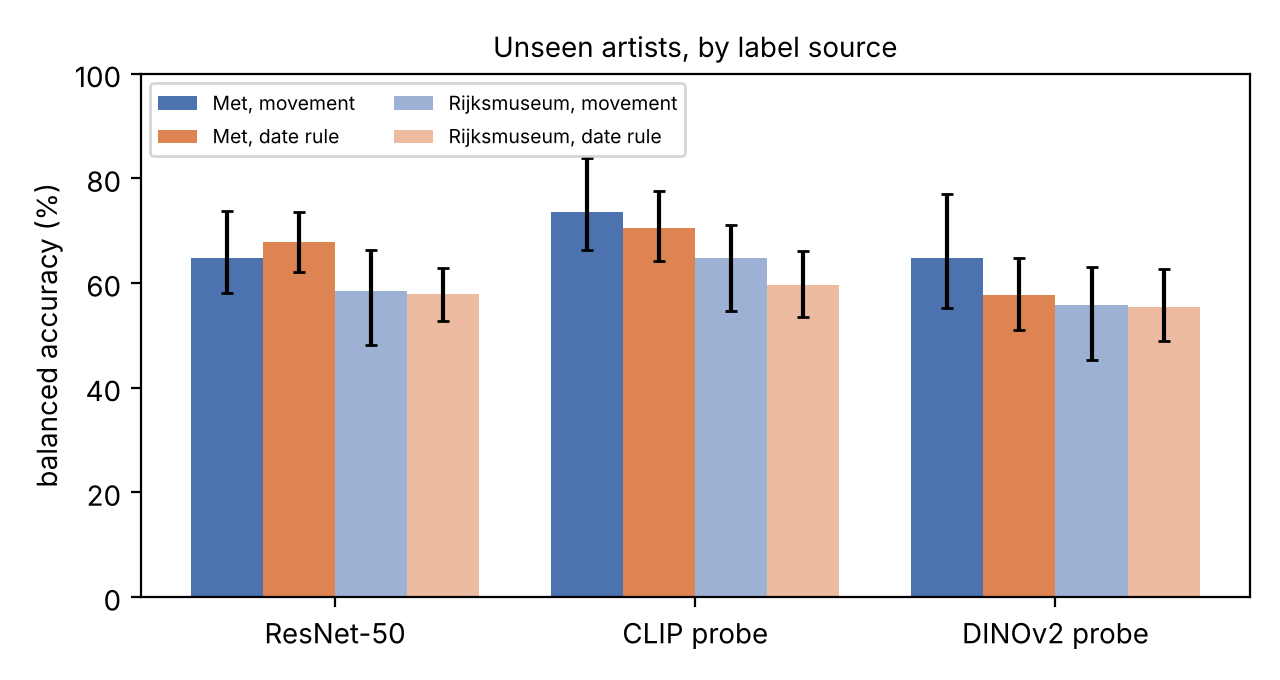
\includegraphics[width=\columnwidth]{figures/label_source.png}
\caption{Balanced accuracy on unseen-artist museum paintings, by how the label was made (four shared styles; painter-level 95\% CI).}
\label{fig:labelsource}
\end{figure}

\textbf{Digitization ablations} (ResNet-50, 3 seeds, test-time changes). Matching each museum's color statistics to WikiArt's changes unseen-artist accuracy by $-$0.1 (Met) and +0.3 (Rijksmuseum); re-saving at WikiArt's JPEG quality changes it by 0.0 and +0.1. A center crop helps the Met by +2.5 $\pm$ 2.5 (noisy) and does nothing at the Rijksmuseum. Degradations hurt WikiArt about as much as the museums or more: grayscale $-$8.9 on WikiArt vs $-$6.2 and $-$3.9; JPEG quality 50 $-$7.4 vs $-$3.7 and $-$2.3; 128\,px $-$5.6 vs $-$6.4 and $-$4.6. So museum scans are not more fragile, there is little gap for a fix to close, and the model relies on color. Because WikiArt is only available at 256\,px and museum images were resized to match, \emph{this design cannot test whether higher resolution would help}.

\textbf{Training-time color changes.} Color jitter during training (brightness and saturation $\pm$20\%, 3 seeds) gives +2.7 at the Met [0.0, 5.0] and +1.2 at the Rijksmuseum [$-$0.6, 3.7], but top-1 accuracy falls by 2--3 points and none of the seed-level t-tests is significant ($p \ge 0.15$). It trades styles rather than improving recognition: Mannerism recall rises 14--18 points while Baroque falls 5--10. Grayscale augmentation ($p = 0.2$, 3 seeds) gives \pend\ (WikiArt), \pend\ (Met) and \pend\ (Rijksmuseum), and its color reliance (normal minus grayscale test images) is \pend\ points against \pend\ for the baseline.

\textbf{CORAL.} Aligning feature covariances (Table~\ref{tab:coral}) changes unseen-artist balanced accuracy by \pend\ to \pend\ points. Compared with the individual fixes above, \pend.

\begin{table}[t]
\centering
\caption{CORAL on frozen features (unseen artists, balanced accuracy, painter-level paired bootstrap).}
\label{tab:coral}
\begin{tabular}{llrrc}
\toprule
Model & Museum & No adapt. & CORAL & Gain [95\% CI] \\
\midrule
CLIP & Met & \pend & \pend & \pend \\
 & Rijks & \pend & \pend & \pend \\
DINOv2 & Met & \pend & \pend & \pend \\
 & Rijks & \pend & \pend & \pend \\
SigLIP & Met & \pend & \pend & \pend \\
 & Rijks & \pend & \pend & \pend \\
\bottomrule
\end{tabular}
\end{table}

\textbf{Calibration.} All models are less calibrated on museum images than on WikiArt test (Table~\ref{tab:record}): ResNet-50 ECE rises from 0.039 to 0.069 (Met) and 0.056 (Rijksmuseum), CLIP from 0.099 to 0.155 and 0.125. The CLIP probe is the most accurate and the most over-confident model. DINOv2 is the exception (0.085 on WikiArt, 0.065 and 0.055 on museums).

% ===========================================================================
\section{RQ2: Few-Shot Fine-Tuning on the Other Museum}

\begin{figure}[t]
\centering
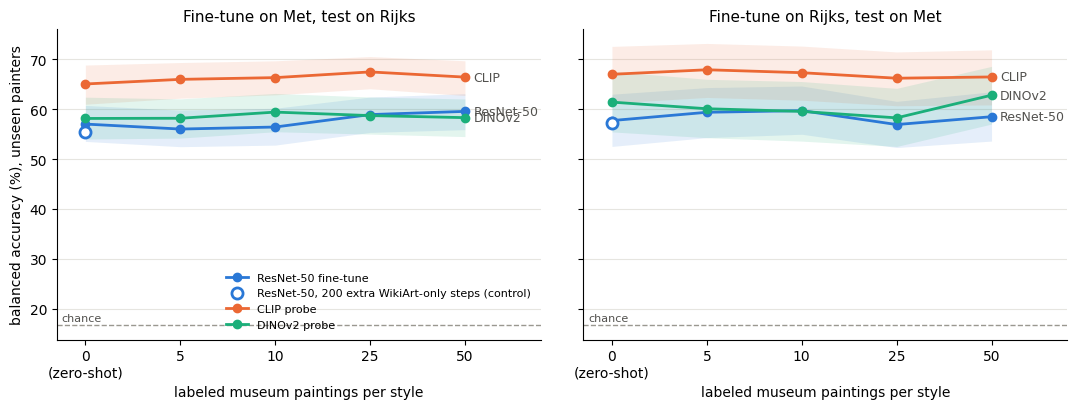
\includegraphics[width=\columnwidth]{figures/rq2_curve.png}
\caption{RQ2 few-shot curves on the fixed test sets (balanced accuracy, mean of 3 seeds, painter-disjoint from WikiArt train and from the source museum).}
\label{fig:rq2}
\end{figure}

\begin{table}[t]
\centering
\caption{RQ2: balanced accuracy at $k=0$ and $k=50$ shots per style; gain with paired bootstrap 95\% CI (3 seeds).}
\label{tab:rq2}
\setlength{\tabcolsep}{3pt}
\begin{tabular}{llrrc}
\toprule
Direction & Model & $k{=}0$ & $k{=}50$ & Gain [95\% CI] \\
\midrule
Met$\to$Rijks & ResNet-50 & 57.0 & 59.5 & +2.5 [$-$0.1, 5.2] \\
($n=2{,}279$) & CLIP probe & 65.0 & 66.4 & +1.4 [$-$1.6, 4.3] \\
 & DINOv2 probe & 58.1 & 58.3 & +0.2 [$-$2.8, 3.0] \\
Rijks$\to$Met & ResNet-50 & 57.7 & 58.5 & +0.8 [$-$2.1, 3.7] \\
($n=424$) & CLIP probe & 67.0 & 66.4 & $-$0.5 [$-$4.2, 3.2] \\
 & DINOv2 probe & 61.4 & 62.8 & +1.4 [$-$2.0, 4.6] \\
\bottomrule
\end{tabular}
\end{table}

Fig.~\ref{fig:rq2} and Table~\ref{tab:rq2} answer RQ2: a few labeled paintings from one museum barely help on the other. None of the 24 gains (3 models $\times$ 2 directions $\times$ 4 values of $k$) is significant; the largest is ResNet-50, Met$\to$Rijksmuseum, $k{=}50$ ($p = 0.06$). The WikiArt-only control (\emph{k0ft}) changes ResNet-50 by $-$1.6 and $-$0.4, so the extra steps alone do not help either. WikiArt test stays at 59--61 after fine-tuning, so there is no forgetting. Per style, the shots move errors between styles rather than removing them: for ResNet-50, Met$\to$Rijksmuseum at $k{=}50$, Romanticism recall rises from 39 to 59 and Mannerism from 40 to 45, while Baroque falls from 59 to 52; ECE doubles from 0.07 to 0.15. The two directions agree, which fits RQ1: there is little museum-specific loss for museum shots to recover.

% ===========================================================================
\section{Failure Analysis}

\begin{figure*}[t]
\centering
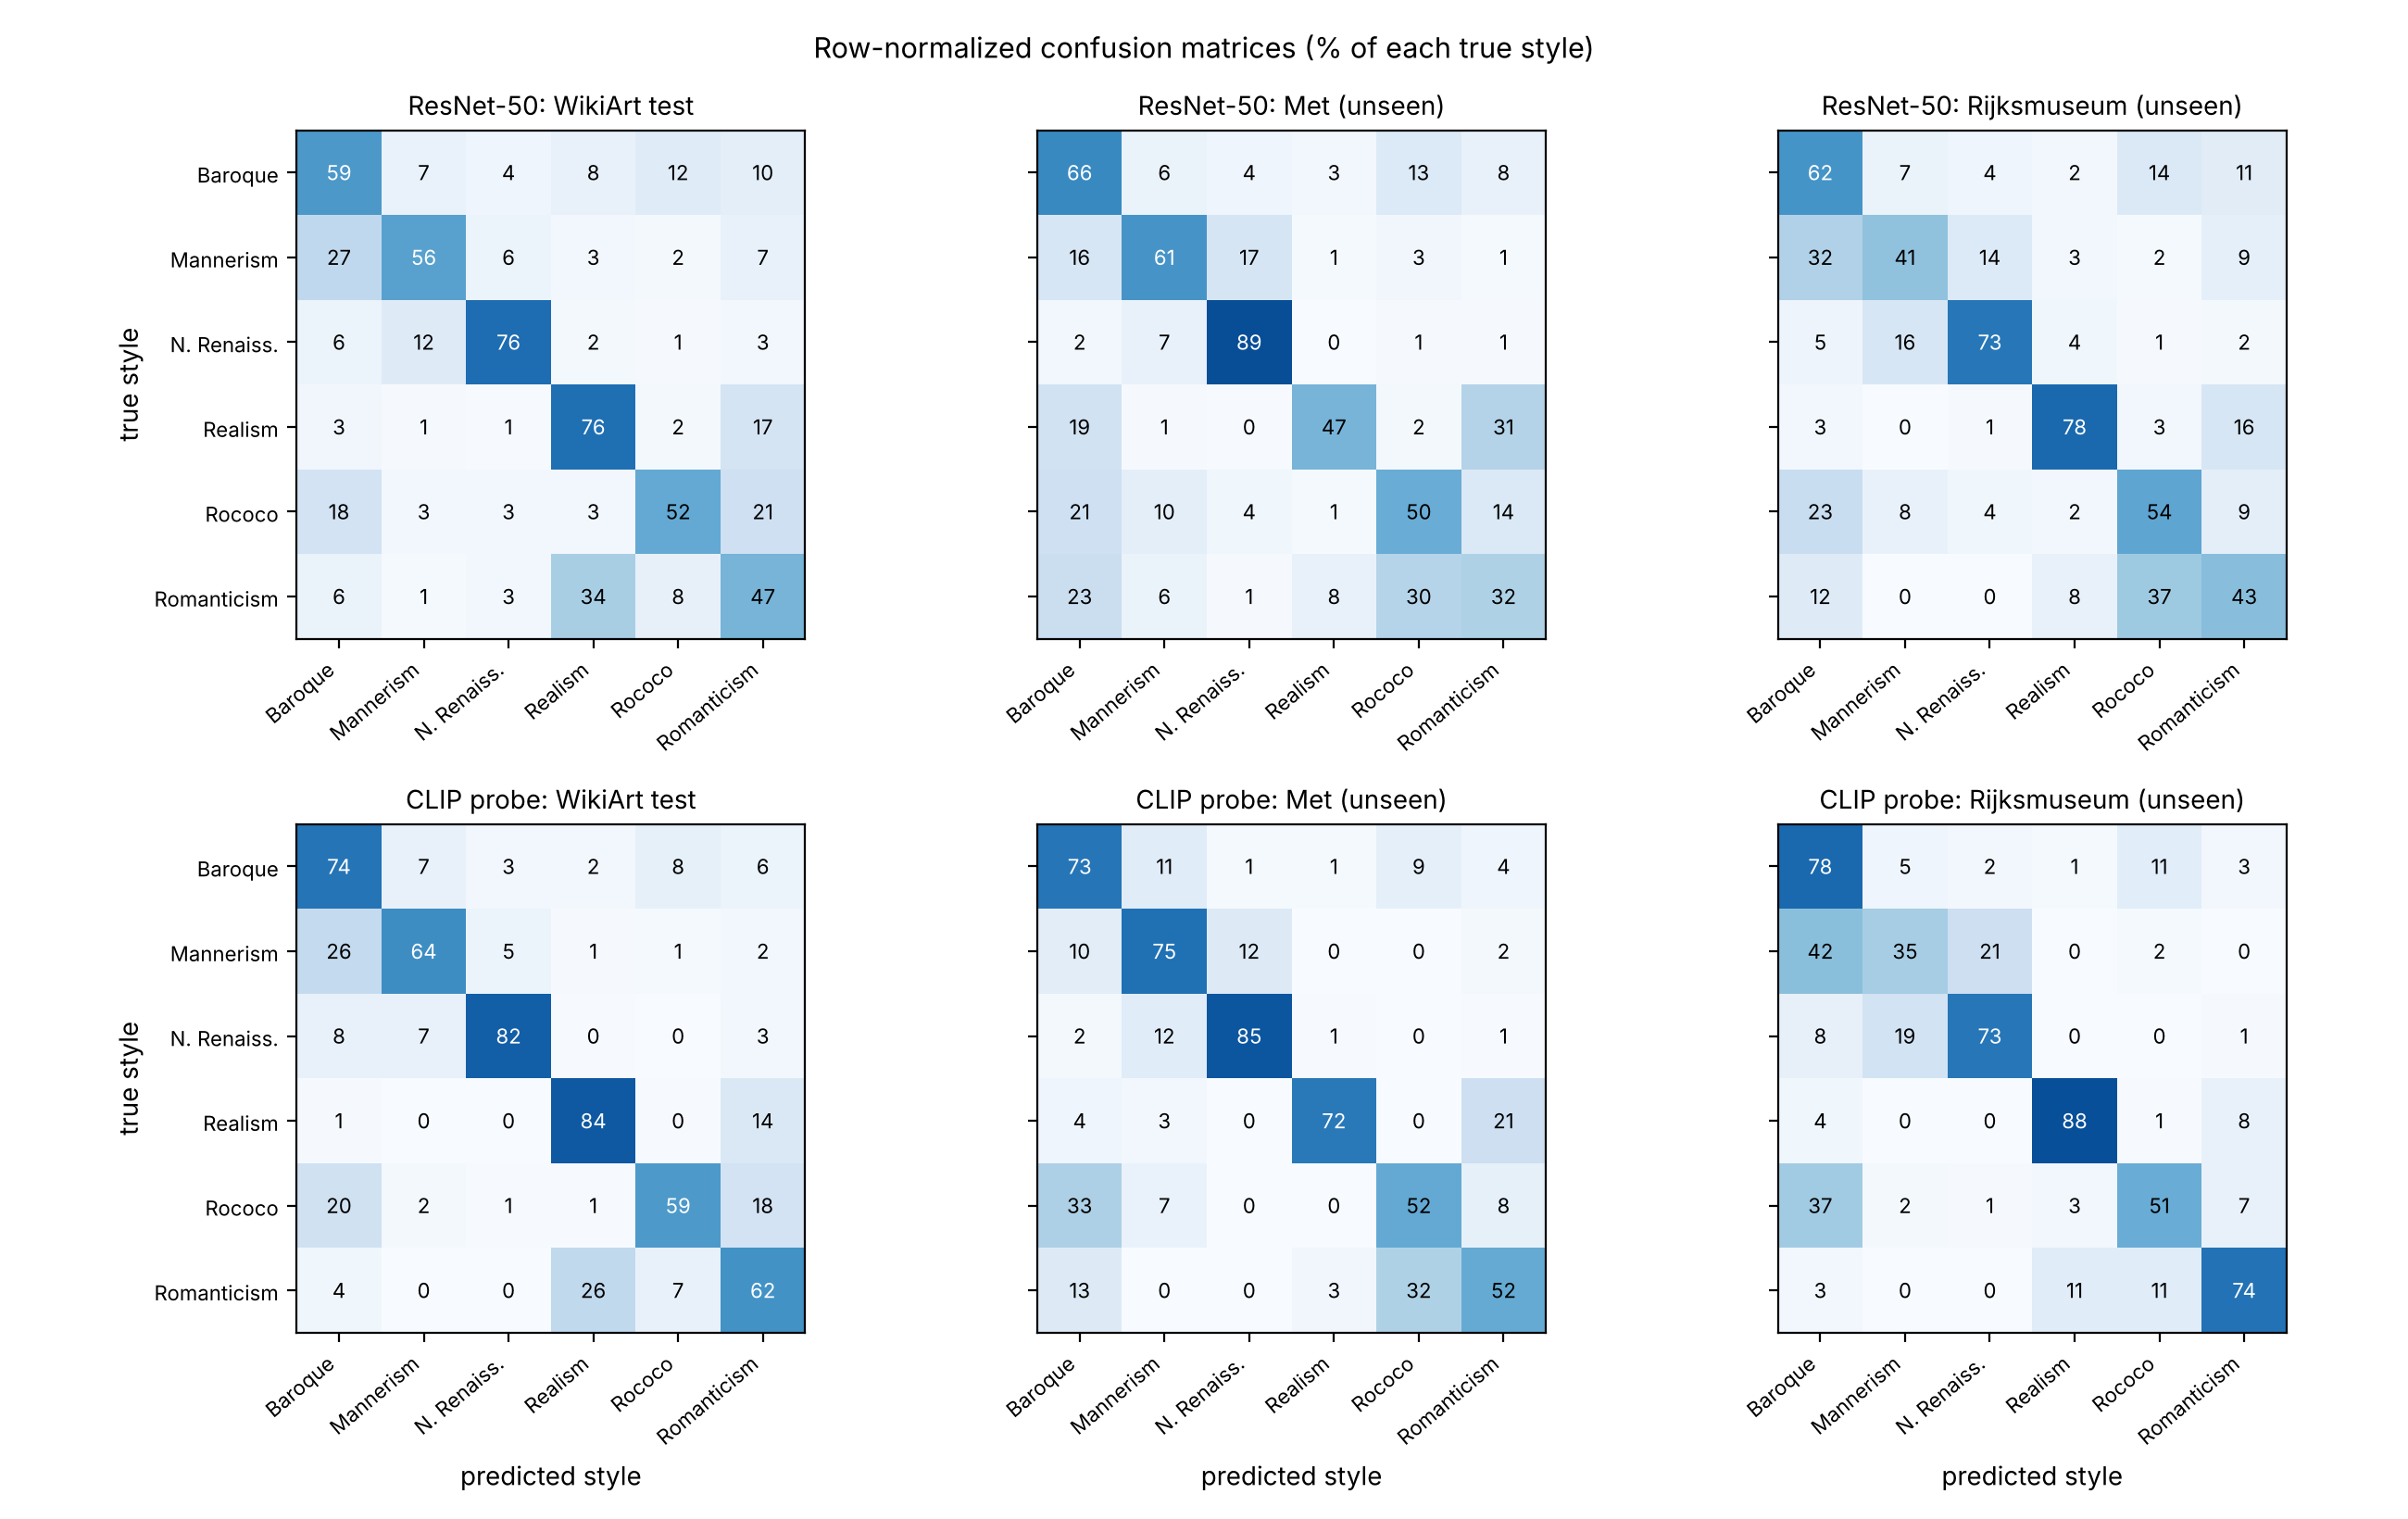
\includegraphics[width=0.9\textwidth]{figures/confusion_matrices.png}
\caption{Row-normalized confusion matrices (\% of each true style). Top: ResNet-50 (3 seeds). Bottom: CLIP probe. Museums: unseen artists.}
\label{fig:confusion}
\end{figure*}

\textbf{Most-confused pairs} (Fig.~\ref{fig:confusion}). The same historical neighbors dominate everywhere. On WikiArt test, Romanticism$\to$Realism (34\% for ResNet-50) and Mannerism$\to$Baroque (27\%) lead. At the Met, ResNet-50 sends Realism to Romanticism (31\%) and Romanticism to Rococo (30\%); CLIP sends Rococo to Baroque (33\%). At the Rijksmuseum, Mannerism$\to$Baroque (32\% ResNet-50, 42\% CLIP) and Rococo$\to$Baroque (23\%, 37\%) lead. These are adjacent periods with shared subjects, so most confusion is historical overlap.

\textbf{Strong and weak styles.} Northern Renaissance transfers best (ResNet-50 recall 89\% at the Met), consistent with its distinctive panel technique and narrow date range. Romanticism is weakest (WikiArt 47\%, Met 32\%, Rijksmuseum 43\%) and is confused with Realism, Rococo and Baroque in both directions: it is defined more by subject and mood than by technique. Met Realism drops from 76\% on WikiArt to 47\%, mostly to Romanticism (31\%). Rococo is confused with Baroque in every set.

\textbf{Tally of confident errors.} We took the 30 most confident wrong predictions per museum (ResNet-50, unseen artists; confidence 0.80--0.96) and assigned each a primary cause and any visible digitization factor. Tags were drafted with AI assistance from contact sheets of the images, titles and dates, and checked by the author against the images (\texttt{results/final/error\_tally.csv}). Of 60 errors, 33 (55\%) sit at a \emph{style boundary}: the painting's date or painter lies near the edge between two styles (for example portraits of 1696--1746 by Largillierre, Rigaud, Kneller or Philip van Dijk labeled Baroque and predicted Rococo). Nine (15\%) are \emph{label problems}: later copies or imitations whose date sends them to the wrong style, such as an 18th-century copy of a 16th-century portrait labeled Rococo by the date rule and predicted Northern Renaissance, or Pieter Brueghel the Younger's 1614 copy of his father's composition labeled Baroque. Eight (13\%) depict another period or are non-European works, seven (12\%) have a digitization or format cause (a triptych with black gaps, an oval or round format, a visible frame, a grisaille), and three have no clear cause. Counting all visible factors, 14 errors show a frame, border or non-rectangular format, 7 a color cast, dark varnish or near-monochrome surface, and 3 an inscription; none show glare, an unusual crop or low resolution. Digitization factors are therefore present in a minority of confident errors and rarely the main cause.

\textbf{Rijksmuseum Mannerism.} Mannerism recall for CLIP is 75\% at the Met but 35\% at the Rijksmuseum (unseen artists), and a closer look at the labels explains why. The 72 Rijksmuseum Mannerism paintings are 63 northern and 7 Italian works (Met: 49 of 59 Italian), while WikiArt's Mannerism training set is led by Tintoretto, Veronese, El Greco, Bronzino and Pontormo. Labels come from the painter's movement (48) or the 1580--1599 northern date rule (24), and 25 are works dated before 1580 whose painter Wikidata lists as Mannerist. By eye, 26 are Mannerist history or allegory paintings (Heemskerck, Wtewael, Cornelis van Haarlem, Goltzius, Spranger), 29 are portraits or group portraits, 6 are grisailles, 6 are Italian religious works and 5 are other subjects. ResNet-50 recognizes the Italian works (83\%) but only 38\% of the northern history paintings (most go to Baroque or Northern Renaissance), 52\% of the portraits and none of the grisailles. The labels follow their rules correctly, but ``Mannerism'' at the Rijksmuseum is a movement-and-date category that looks different from the Italian Mannerism WikiArt teaches. This is a construct-validity issue, not a digitization effect. The visual check was done in the same AI-assisted way and confirmed by the author (\texttt{results/final/rijks\_mannerism.csv}).

% ===========================================================================
\section{Merged Styles (an Option, Not a Replacement)}

The instructor asked for higher accuracy. Six-way style recognition on unseen painters is limited by real overlap between neighboring styles, so we also report scores with styles merged after prediction into four groups (Renaissance = Northern Renaissance + Mannerism, Baroque/Rococo, Romanticism, Realism; chance 25\%) and three eras (Renaissance, Baroque/Rococo, 19th century; chance 33\%). Merging changes the research question, so Table~\ref{tab:merged} sits next to the six-style results and does not replace them.

\begin{table}[t]
\centering
\caption{Balanced accuracy (\%) with six styles and after merging (museums: unseen artists). Final ensemble: one run.}
\label{tab:merged}
\setlength{\tabcolsep}{3pt}
\begin{tabular}{llrrr}
\toprule
Model & Test set & 6 styles & 4 groups & 3 eras \\
\midrule
ResNet-50 & WikiArt test & 61.1 & 67.4 & 78.4 \\
 & Met & 57.5 & 59.7 & 78.3 \\
 & Rijksmuseum & 58.2 & 67.7 & 80.7 \\
\midrule
CLIP probe & WikiArt test & 70.9 & 76.8 & 84.7 \\
 & Met & 68.2 & 74.3 & 86.2 \\
 & Rijksmuseum & 66.4 & 82.6 & 87.3 \\
\midrule
Final ensemble & WikiArt test & 78.3 & 81.7 & 92.1 \\
 & Met & 70.3 & 70.4 & 87.0 \\
 & Rijksmuseum & 71.0 & 80.6 & 90.9 \\
\bottomrule
\end{tabular}
\end{table}

With three eras the best model reaches 87--91\% balanced accuracy on unseen-artist museum paintings. Top-3 accuracy on six styles is 96--99\% for the foundation models, but its chance level is 50\%, so it is not a fair headline. Upper-90s top-1 accuracy on six styles for unseen painters is not supported by our data, and we did not pursue it by relaxing the artist-disjoint split.

% ===========================================================================
\section{Threats to Validity}
\label{sec:threats}

\textbf{Internal.} (i) \emph{Style mapping}: museum labels are derived, not catalogued, and about half come from a date rule; Section~\ref{sec:rq1} shows no significant difference by label source, but the intervals are wide. (ii) \emph{Overlap removal}: we removed 721 museum paintings found in WikiArt and checked 60 pairs by eye, but near-copies that escape perceptual hashing could remain. (iii) \emph{Contamination}: CLIP's web pretraining data very likely includes WikiArt and museum images, and DINOv2's curated data and SigLIP's may as well; their scores may be flattering. The ImageNet-initialized ResNet-50 has no such exposure, so it is the cleanest test of transfer, and it shows the same small gap. (iv) \emph{Small WikiArt test}: 81 painters, with only 3--8 for some styles, so in-domain per-style recall depends on a few artists.

\textbf{External.} Both museums are Western and both are professionally digitized. We did not add an in-gallery photo set: collecting licensed or self-taken gallery photos was not feasible in the course timeline, so our results cannot separate ``different digitization pipeline'' from ``photographed in the room'' and do not apply to visitor photos. That set is future work.

\textbf{Construct.} ``Style'' means a community tag on WikiArt and a movement-or-date rule for the museums. The Rijksmuseum Mannerism result shows that these definitions can disagree even when each is applied correctly.

\textbf{Comparability with published results.} We did not use the standard 27-style WikiArt release, because most of its images have no artist, which makes an artist-disjoint split impossible, and published results on it use random splits that share artists (worth about 10 points~\cite{ashton2026}). Our six-style, artist-disjoint numbers are therefore not directly comparable with published 27-style accuracies. We did not train on the 27-style subset with known artists, which remains a useful comparison.

% ===========================================================================
\section{Ethics, Licensing and Reproducibility}

\textbf{Ethics and licensing.} WikiArt contains copyrighted modern works and its images are for non-commercial research only, so we release image IDs, source URLs and label maps, not images. Met Open Access and Rijksmuseum images are public domain or CC0; Wikidata is CC0. Fig.~\ref{fig:examples} shows only public-domain works. No personal data is used. \textbf{Use of AI tools}: an AI assistant drafted label verdicts (checked blind by the author), drafted the error and Mannerism tags (checked by the author), and helped with code and editing; all results were run and checked by the author.

\textbf{Reproducibility.} The repository contains all code and Colab notebooks; the artist-disjoint split (SHA-256 prefix \texttt{d5bb835c8cd9526a}); the label, rule and source for all 6,909 museum paintings; Met and Rijksmuseum object IDs with export dates; the overlap (721) and near-duplicate (425) lists; seeds (split 42, training 1--3); model, probe, ablation and few-shot settings; library versions (training: Python 3.13, PyTorch 2.11); and the prediction file behind every table. \texttt{src/final\_analysis.py} recomputes Tables~\ref{tab:record}--\ref{tab:balanced} from the prediction files without a GPU.

% ===========================================================================
\section{Conclusion}

A style classifier trained on WikiArt loses only a few points on professional digitizations from the Met and the Rijksmuseum: 2--5 points of balanced accuracy, with intervals that include zero and rule out a loss above about 10 points. Whether the model knows the artist matters more, about 12 points at the Met for every model. A few museum paintings from one museum do not help on the other. Most confident errors come from neighboring styles and from how style labels are defined, so better labels, not better digitization fixes, are the most promising next step, together with an in-gallery photo test set.

\section*{Acknowledgment}
The project idea and its two-question framing come from Mashfika Jahan and Yisihaq Yemiu, used with their agreement. We thank Dr.~Suboh Alkhushayni for detailed feedback, and the Metropolitan Museum of Art, the Rijksmuseum, WikiArt and Wikidata for open data.

\bibliographystyle{IEEEtran}
\bibliography{refs}

\end{document}
